\documentclass[tikz,border=3pt]{standalone}
\usepackage{newtxtext}
\usetikzlibrary{arrows.meta,fit,positioning}

\begin{document}
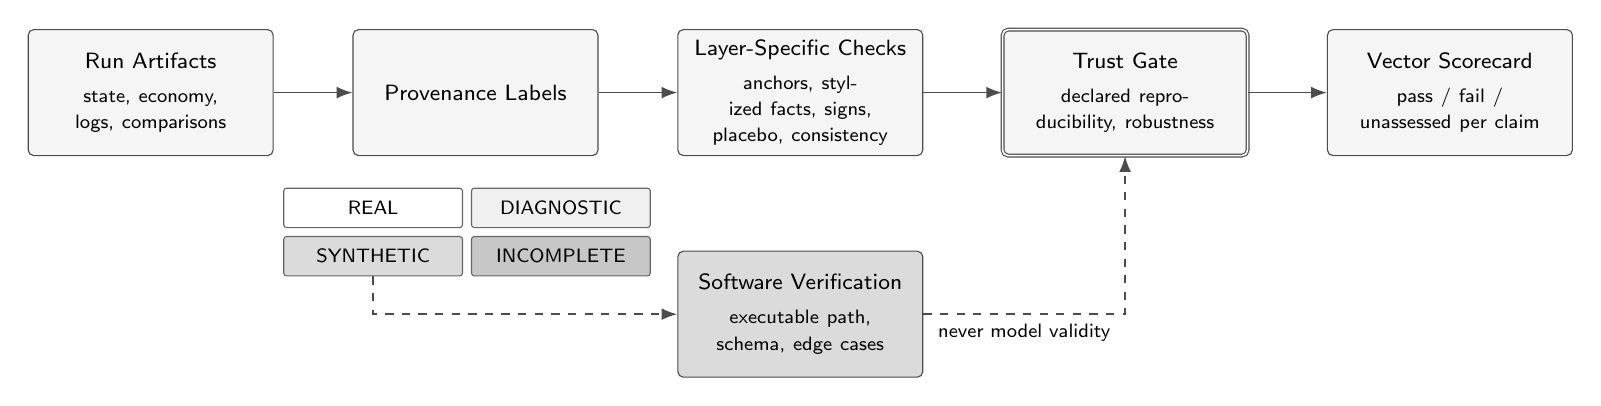
\begin{tikzpicture}[
  font=\sffamily\footnotesize,
  box/.style={draw=black!70, rounded corners=2pt, minimum height=16mm,
    text width=29mm, align=center, inner sep=3pt, fill=black!4},
  labelbox/.style={draw=black!60, rounded corners=1pt, minimum height=5mm,
    text width=22mm, align=center, inner sep=1pt, font=\sffamily\scriptsize},
  arrow/.style={-{Latex[length=2mm]}, semithick, draw=black!70},
  reject/.style={-{Latex[length=2mm]}, dashed, semithick, draw=black!70}
]
  \node[box] (artifacts) {Run Artifacts\\[1mm]\scriptsize state, economy, logs, comparisons};
  \node[box, right=10mm of artifacts] (provenance) {Provenance Labels};
  \node[box, right=10mm of provenance] (checks) {Layer-Specific Checks\\[1mm]\scriptsize anchors, stylized facts, signs, placebo, consistency};
  \node[box, right=10mm of checks, double] (gate) {Trust Gate\\[1mm]\scriptsize declared reproducibility, robustness};
  \node[box, right=10mm of gate] (scorecard) {Vector Scorecard\\[1mm]\scriptsize pass / fail / unassessed per claim};

  \draw[arrow] (artifacts) -- (provenance);
  \draw[arrow] (provenance) -- (checks);
  \draw[arrow] (checks) -- (gate);
  \draw[arrow] (gate) -- (scorecard);

  \node[labelbox, fill=white, below=4mm of provenance, xshift=-13mm] (real) {REAL};
  \node[labelbox, fill=black!6, right=1mm of real] (diagnostic) {DIAGNOSTIC};
  \node[labelbox, fill=black!14, below=1mm of real] (synthetic) {SYNTHETIC};
  \node[labelbox, fill=black!22, right=1mm of synthetic] (incomplete) {INCOMPLETE};

  \node[box, below=12mm of checks, fill=black!14] (software) {Software Verification\\[1mm]\scriptsize executable path, schema, edge cases};
  \draw[reject] (synthetic.south) |- (software.west);
  \draw[reject] (software.east) -| node[pos=.25, below, font=\sffamily\scriptsize]
    {never model validity} (gate.south);
\end{tikzpicture}
\end{document}
